\section{Model Selection and Comparison}\label{apdx:methodology}
\subsection{Model Selection Process}\label{apdx:model_selection}

In the initial stage of the model selection process, I considered models of the following form:
\begin{equation}\label{eq:generalized_equation}
    g(C_i) = \alpha^{s}_{t} + f(E_i, P_i) + \varepsilon_i
\end{equation}

The constant $\alpha^{s}_{t}$ is superscripted by sector $s$ (residential and non-residential) and subscripted by year $t$. This allows for the constant to vary over time, separately for each sector, to capture changes in productivity over time separately from effects of system size, which are captured by $f(\cdot)$. Below, in \ref{apdx:time_var_coef}, I consider the possibility that coefficients governing $f(\cdot)$ may also vary over time.

The functions $g(\cdot)$ and $f(\cdot)$ represent any of several possible transformation of the variables. For $g(\cdot)$, I consider no transformation of installed cost, cost per kWh, the natural log of installed cost, and the natural log of cost per kWh. Models with different transformations of the dependent variable cannot be validly compared by several common measures of goodness-of-fit. Root-mean-square error (RMSE) is measured in the unit of the dependent variable, so one cannot compare \textit{e.g.} errors measured in log dollars with errors measured in dollars per kWh. A non-linear transformation of the dependent variable changes the distribution of the errors, so neither can one use mean absolute percentage error (MAPE), either. R\textsuperscript{2} is not appropriate when comparing models with different, non-linear transformations of the dependent variable. For example, the R\textsuperscript{2} of a model of installed cost represents the percentage of squared deviations from the mean of total installed cost that is explained by the regressors, whereas the R\textsuperscript{2} of a model of cost per kWh represents the percentage of squared deviation from mean of cost per kWh. The structure of the variance of total installed cost is radically different from the structure of the variance of installed cost per kWh.

I instead compare the models on the basis of Akaike Information Criterion (AIC) \citep{akaike1974}:

\begin{equation}
AIC = 2k - 2\ln(\widehat{L})
\end{equation}

where $k$ is the number of parameters and $\widehat{L}$ is the maximum of the model's likelihood function. AIC can be described as the ``information loss'' that results from the representation of the data by a model in a manner analagous to the loss of information resulting from the representation of a territory by a map. When comparing models based on the same underlying data, lower relative values of AIC correspond to less loss of information. Given two models (A) and (B), the quantity $\exp((AIC_A-AIC_B)/2)$ expresses the relative likelihood of model (B) compared to model (A).

For $f(\cdot)$, I consider a linear combination of energy and power, a quadratic combination ($E_i$, $E^2_i$, $P_i$, $P^2_i$, $E_i \times P_i$), a linear combination of log energy and log power, and a quadratic combination of the log-transformed variables ($\ln(E_i)$, $\ln(E_i)^2$, $\ln(P_i)$, $\ln(P_i)^2$, $\ln(E_i) \times \ln(P_i)$). As there are four transformations of the dependent variable and four transformations of the independent variable, I consider a total of sixteen candidate models and estimate each one on the SGIP sample. In computing the AIC of each model, I account for the transformed dependent variables by adjusting the AIC per the method described by \citet[p. 224]{akaike1978}. 

The composition of this paper began in late 2021. The original model selection analysis and decision was performed with the available data as of January 4\Xth, 2022. The results that follow are based on data spanning 2013 to 2021. The results do not change if data from year 2022 are incorporated.

\subsection{Comparison of Model Fit}\label{apdx:model_comparison}

\begin{table}[h]
\centering
\begin{tabular}{|c|cccc|}\hline
Independent & \multicolumn{4}{c|}{Dependent Variable}  \\ \cline{2-5}
Variables &  \$  \Tstrut  &  \$/kWh  & ln(\$) & ln(\$/kWh)  \\\hline
level, linear     &   $7.32 \times 10^5 $     &  $6.03 \times 10^5 $ & $6.03 \times 10^5 $  &  $5.75 \times 10^5 $  \\
level, quadratic   &   $7.25 \times 10^5 $     &  $6.02 \times 10^5 $ & $6.01 \times 10^5 $  &  $5.75 \times 10^5 $  \\
log, linear     &   $7.78 \times 10^5 $ &    $6.00 \times 10^5$  & $5.72 \times 10^5 $ & $5.72 \times 10^5 $ \\
log, quadratic  &   $7.57 \times 10^5 $ &    $5.98 \times 10^5$  & $5.71 \times 10^5 $ & $5.71  \times 10^5 $ \\\hline
\end{tabular}
\caption{Akaike Information Criteria of Sixteen Models of Installed Cost of BTM BESS.}\label{tab:SGIP_AIC} 
\end{table}

The values of AIC for each of the sixteen candidate models are displayed in Table \ref{tab:SGIP_AIC}. Careful readers will note that there are two pairs of models in Table \ref{tab:SGIP_AIC} with apparently equal AIC. For the models that log-transform both the dependent and independent variables, the decision of whether to set the dependent variable as log total cost or log cost per kWh is essentially inconsequential. The two representations are nearly algebraically equivalent. After examining the values of AIC to more significant digits, I determined that the models with log total cost slightly outperform the corresponding models with log cost per kWh. Furthermore, I prefer the models that take log total cost as the dependent variable because they correspond to functional forms in widespread use, with names established by convention.

The model corresponding to row 3, column 3 of Table \ref{tab:SGIP_AIC} is a case of the Cobb-Douglas \citep{cobbdouglas1928} functional form:

\begin{equation}
    \ln(C_i) = \alpha^{s}_{t} + \beta_1 \ln(E_i) + \beta_2 \ln(P_i) + \varepsilon_i \tag{\ref{eq:CD}}
\end{equation}

The model corresponding to row 4, column 3 is a case of the translog \citep{kmenta1967} functional form:

\begin{align}
    \ln(C_i) = &\alpha^{s}_{t} + \beta_1 \ln(E_i) + \beta_2 \ln(P_i) + \gamma_1 \ln(E_i)^2 + \gamma_2 \ln(P_i)^2 \tag{\ref{eq:TL}} \\
		 & + \gamma_3 \ln(E_i) \ln(P_i) + \varepsilon_i \notag
\end{align}

The comparison of AIC indicates unambiguously that a translog relationship between installed cost, energy, and power minimizes the information loss among the sixteen candidate models. Before finalizing the model selection decision, I gave further consideration to the Cobb-Douglas model. Cobb-Douglas is parsimonious in parameters and easy to interpret. In light of its greater number of parameters, the translog model presents a risk for overfitting relative to a Cobb-Douglas model. Because the two models have the same dependent variable, they can be compared on the basis of root mean squared error (RMSE), mean absolute error (MAE), and adjusted-R\textsuperscript{2} and their information criteria can be compared without an adjustment for transformation of the dependent variable. The statistics in Table \ref{tab:CD_vs_TL} indicate that the translog provides a statistically significant---albeit practically trivial---improvement in goodness-of-fit and predictive accuracy relative to Cobb-Douglas by several standard measures. If the translog model were overfit, it would exhibit a larger RMSE than the RMSE of the Cobb-Douglas model under cross-validation. Instead, the cross-validated RMSE of the translog model is marginally smaller.

\begin{table}[h]
\begin{tabular}{lccc}
\hline
                               & \multicolumn{2}{c}{Model} & \multirow{2}{*}{\begin{tabular}[c]{@{}c@{}}Preferred\\ Model\end{tabular}} \\ \cline{2-3}
                               & Cobb-Douglas  & Translog  &                                                                            \\ \hline
Akaike Information Criterion   & 6,442          & 5,601      & Translog                                                                   \\
Bayesian Information Criterion & 6,608          & 5,792       & Translog                                                                   \\
cross-validated RMSE (k = 10)           & 0.331          & 0.326      & Translog                                                                   \\
cross-validated MAE (k = 10)           & 0.231          & 0.219      & Translog                                                                   \\
adjusted R\textsuperscript{2}                    & 0.883         & 0.886      & Translog                                                                    \\ \hline
\end{tabular}
\caption{Model Comparison of Cobb-Douglas and Translog.}\label{tab:CD_vs_TL}
\end{table}

The two models do not differ meaningfully in their predictions for BTM BESS with a discharge duration within the domain of the most common values. Figures \ref{fig:CD_vs_TL_resids}a and \ref{fig:CD_vs_TL_resids}b present the residuals from estimating Cobb-Douglas and translog models with the SGIP sample. In orange, I plot the lowess curve \citep{cleveland1979} of the residuals to highlight durations where the residuals of each model depart from an expectation of zero. Visual inspection suggests that the Cobb-Douglas model underestimates the cost (i.e., generates a prediction with a positive residual) of BTM BESS with discharge durations less than one hour and more than three. Between one and three hours, the distribution of residuals is nearly identical and centered on zero.

\begin{figure}[h]
\centering
	\subfloat[\centering Cobb-Douglas.]{{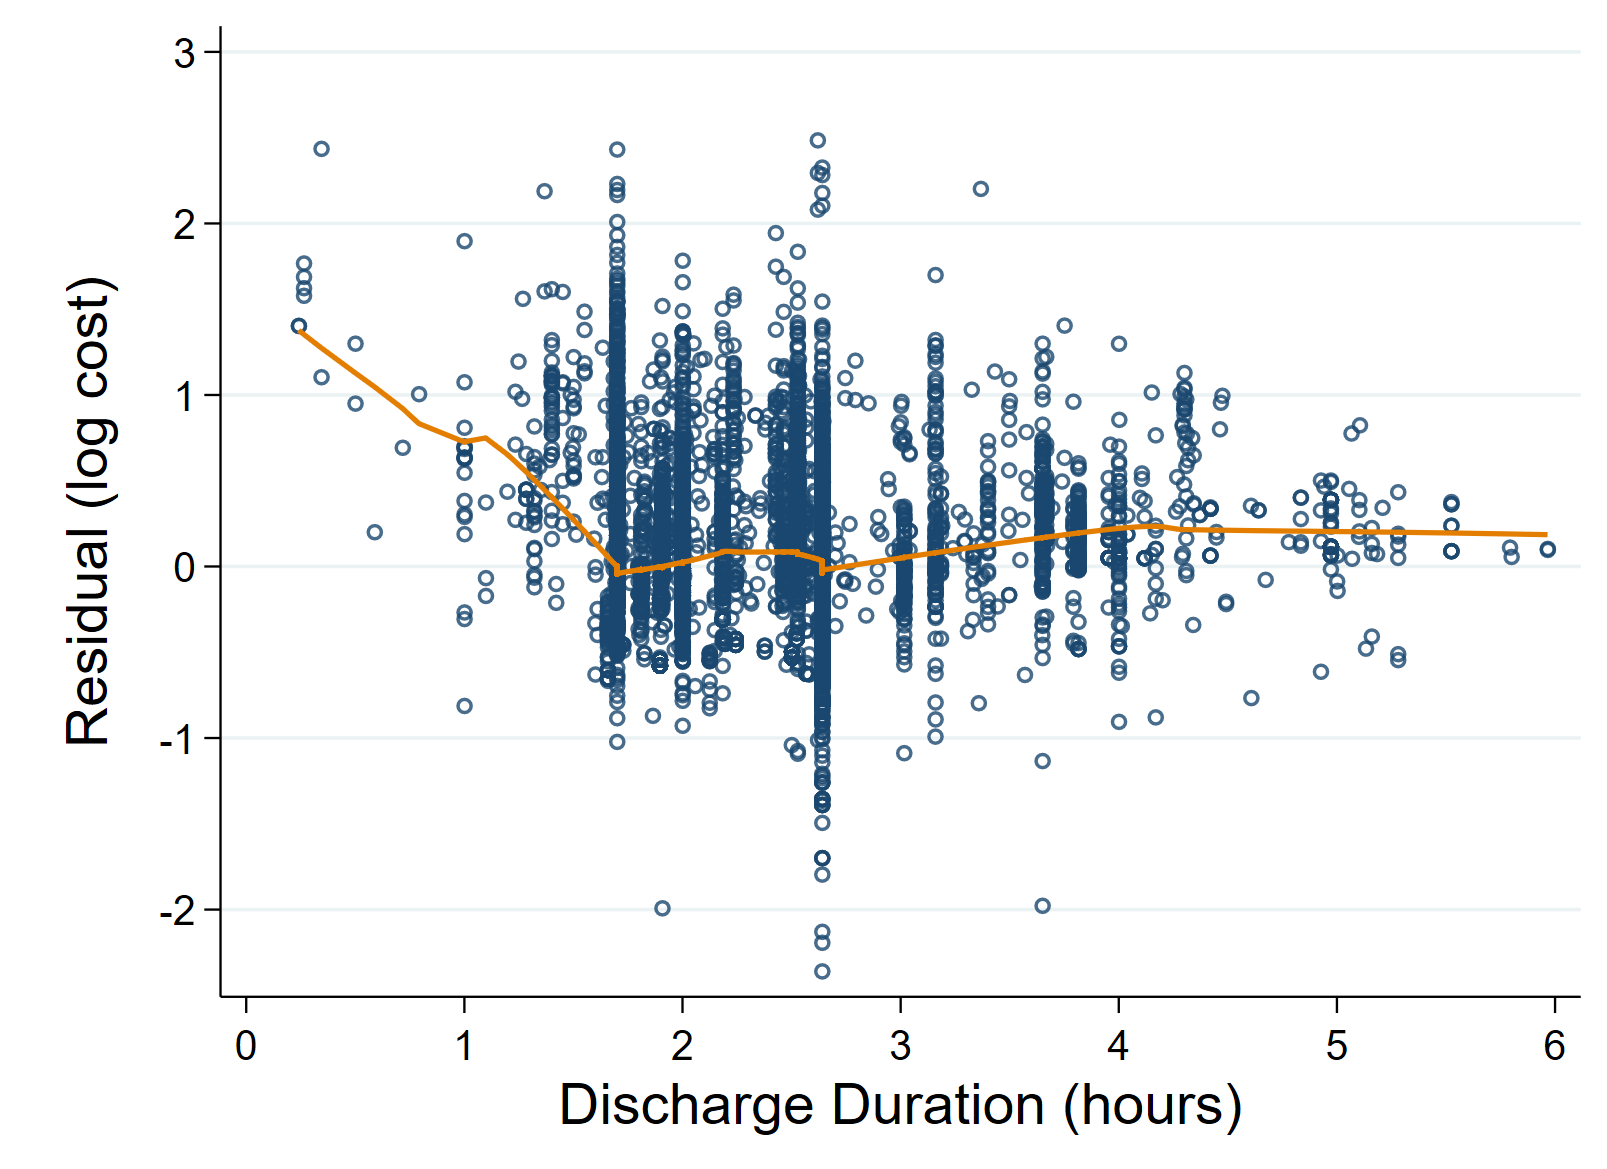
\includegraphics[width=0.5\textwidth]{CA_SGIP/cobb_douglas_resids.png}}}
	\subfloat[\centering Translog.]{{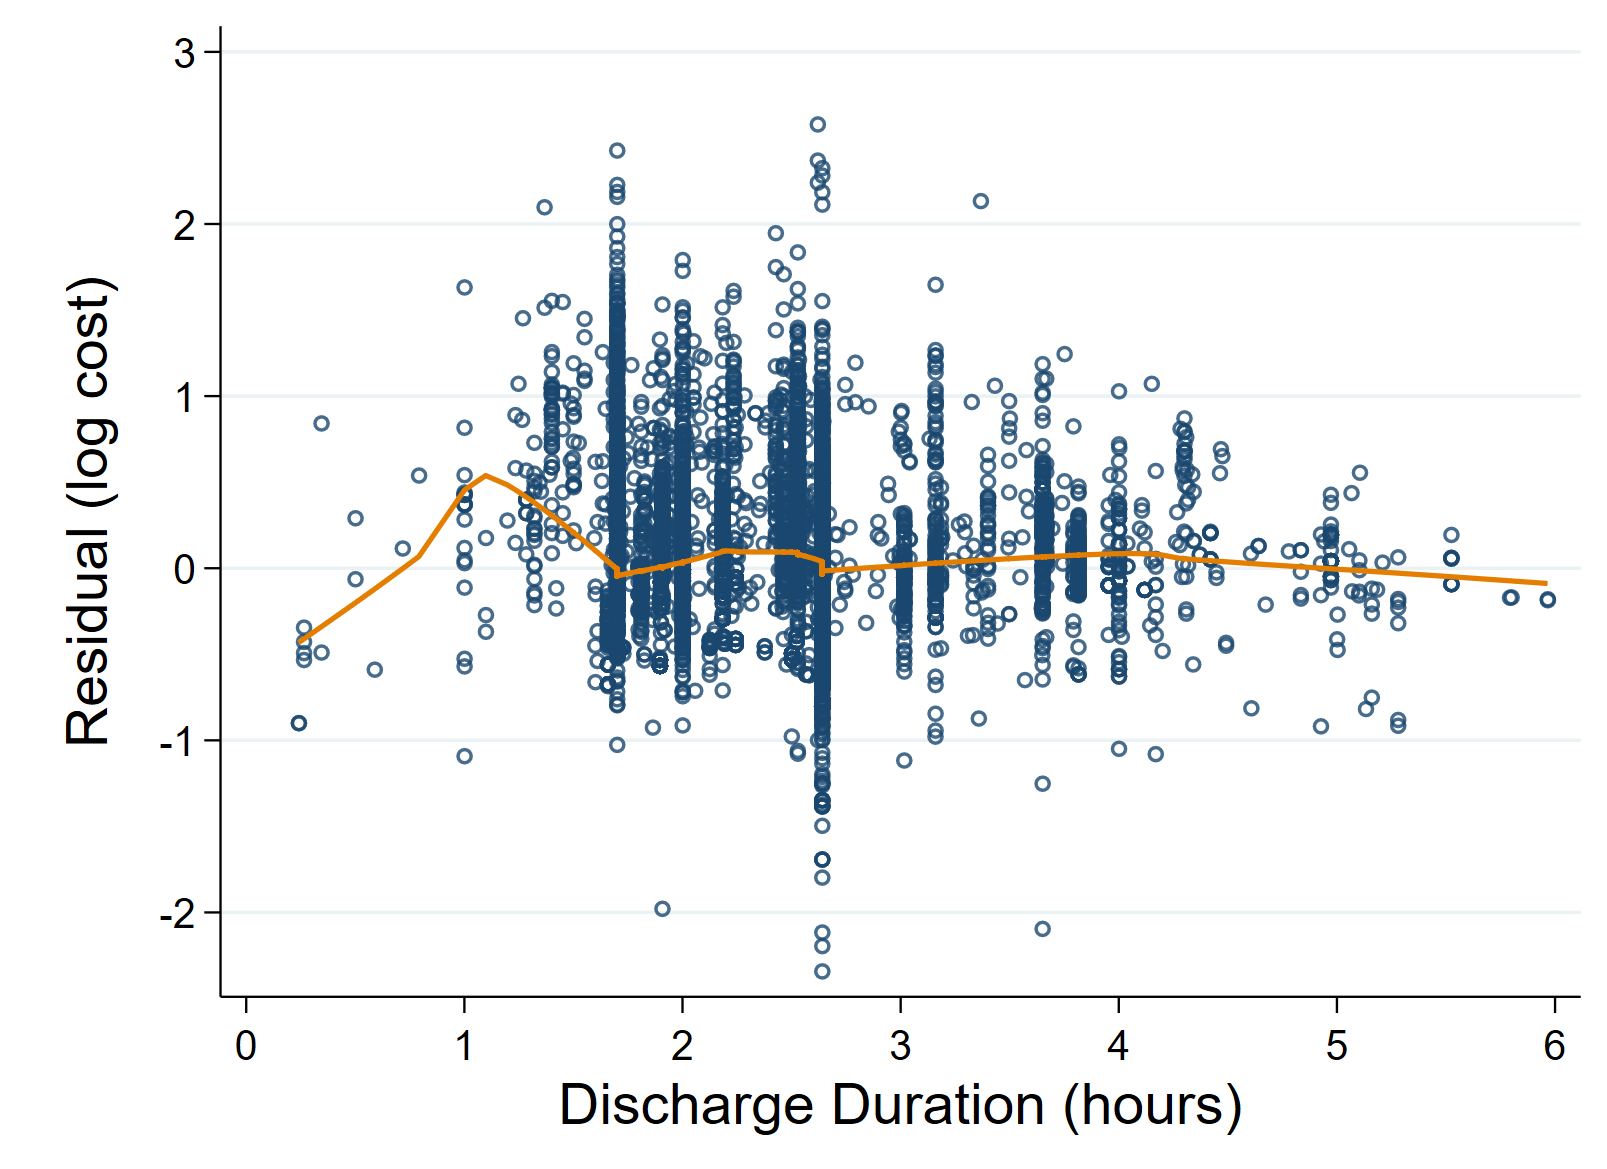
\includegraphics[width=0.5\textwidth]{CA_SGIP/translog_resids.png}}}
\caption{Comparison of Residuals from Estimation of Cobb-Douglas and Translog Models on SGIP Sample.}\label{fig:CD_vs_TL_resids}
\end{figure}

This result is likely related to the fact that 96.3\% of observations in the SGIP sample have discharge durations falling between 1.699 (corresponding to the LG RESU10, 17.1\% of the sample) and 2.64 hours (corresponding to the Tesla Powerwall 2, 62.4\% of the sample), inclusive.\footnote{SGIP reports the name of the battery manufacturer, but not the name of the battery model, which I have inferred. The discharge durations are computed from the SGIP data. SGIP requires project developers to report the energy capacity in terms of ``usable AC energy,'' so these values will not conform to calculations performed with nominal DC or usable DC values reported by the manufacturers.} Hence, the estimated parameters of both models are tightly calibrated to generate unbiased predictions within this range, whereas the residuals outside it are more liable to deviate from an expected value of zero.

A related fact is that there is extremely strong collinearity of energy and power in the SGIP data: the coefficient of correlation is 0.946. Hence, there is limited statistical leverage by which to reliably estimate the independent marginal effect of energy and power, especially outside of the narrow range of commonly observed discharge durations. This clouds the model selection decision because the two models generate very different predictions regarding marginal cost. Whereas the estimated parameters of a Cobb-Douglas model translate to a diminishing marginal cost of energy capacity, the estimated parameters of the translog model translate to an increasing marginal cost of energy capacity. I adjudicate between these competing predictions in the next section.

\subsection{Marginal Cost of Energy Capacity: Cobb-Douglas vs. Translog}\label{apdx:mc}

I investigate the possibility of overfitting by evaluating the extent to which the translog function extrapolates poorly outside the range of the most common discharge durations (1.699 to 2.64 hours). The parameters $\gamma_1$, $\gamma_2,$ and $\gamma_3$ enable curvature in the surface of best fit in the Cartesian space defined by $(\ln(E), \ln(P), \ln(C))$; curvature which marginally improves model fit for ratios of energy to power within the range of the most common values could easily be invalid outside that range. To test this hypothesis, I estimate several Cobb-Douglas models---flat surfaces of best fit in $(\ln(E), \ln(P), \ln(C))$---within restricted sample domains of discharge duration and compare the resulting estimates of marginal cost. 

It is possible that there exist omitted variables correlated with the discharge duration. In particular, manufacturers may differ in their pricing for reasons unrelated to discharge duration, yet pricing and discharge duration may be correlated. I test this hypothesis in two ways: first, I re-estimate Eq. \ref{eq:TL} with an additional set of fixed effects by manufacturer. Second, I restrict the sample domains and then test the sensitivity of the results to inclusion or exclusion of the two most common discharge durations (1.699 and 2.64 hours). These discharge durations are closely associated with the two most dominant manufacturers (LG and Tesla, respectively) in the sample.

In Table \ref{tab:MC_estimates}, I present estimates of the marginal cost of energy capacity for a 5 kW residential BESS under different model specifications. Several conclusions emerge. The first is that Eq. \ref{eq:CD} model does not generate valid predictions of marginal cost (which are presented in row 3) across the full sample domain of discharge durations. All other models agree that there are an increasing marginal costs of energy capacity. The Cobb-Douglas functional form requires that marginal cost of a variable must diminish so long as the exponent on that variable is less than one. This finding improves confidence that the translog model is appropriate---there is indeed curvature in the surface of best fit in $(\ln(E), \ln(P), \ln(C))$.

Regarding the matter of negative marginal costs found in the baseline translog model, that result nearly vanishes when manufacturer fixed effects are included. If we examine the two Cobb-Douglas models restricted to low discharge durations, we see that the negative marginal costs disappear when LG RESU 10s (1.699 hours) are excluded from the sample domain. This implies that the LG RESU 10 has lower costs than systems with shorter discharge durations for reasons unrelated to the extra energy capacity. This may reflect LG's well-established supply chain and economies of scale in the volume of batteries it manufactures. 

When considering the higher range of discharge durations, introducing manufacturer fixed effects to the translog model does not eliminate the finding of increasing marginal costs; if anything, the slope is steeper. If we limit the restrict the sample to the longer durations and estimate a Cobb-Douglas model,  exclusion of the Tesla Powerwall 2 (and any other BESS with the same discharge duration) does reduce the steepness of the marginal cost curve. This implies that the Tesla Powerwall 2 is cheaper than would be predicted on the basis of it discharge duration; given its over-representation in the sample, it distorts the shape of the marginal cost curve.

Given these conclusions, it may seem logical to add manufacturer fixed effects to the model. However, I reject this approach on the grounds that there is good reason to expect that the relative costs of competing manufacturers are liable to change over time in unpredictable ways. A firm could discover a new innovation or scale up the volume of its manufacturing; supply chain issues could increase the costs of some firms more than others; a new firm could enter the market for which no fixed effect has been estimated. As can be plainly seen in Figure \ref{fig:TSLA_cost_adv}, Tesla's cost advantage relative to its competitors has waxed and waned over time. Therefore, I reject the inclusion of manufacturer fixed effects in Eq. \ref{eq:predict_TL}.

The sensitivity of the marginal cost estimates to model specification underscores the need for more project-level data on BTM BESS with greater dispersion in the ratio of energy to power. Given the data currently available for this study, the present estimates of the marginal cost of energy capacity have uncertain validity for BTM BESS with discharge durations outside the range [1.699, 2.64] hours. Considering the balance of the evidence, I argue that the translog model best fits the currently available data.

\begin{landscape}
\begin{table}[h]
\centering
\begin{tabular}{ccc|cccccc}
\hline
\multirow{2}{*}{Model}    & \multirow{2}{*}{\begin{tabular}[c]{@{}c@{}}Sample Domain\\ (hours)\end{tabular}}     & \multirow{2}{*}{N} & \multicolumn{6}{c}{Discharge Duration (hours)} \\\cline{4-9}
                               &                                     &                                       & 1    & 2    & 3  & 4    & 5    & 6   \\ \hline
Translog (Baseline)            & {[}0, 6{]}                    & 26,154                                     & -\$344   & \$692    & \$1,135    & \$1,578    & \$2,089    & \$2,689   \\
Translog (Mfr. F.E.s) & {[}0, 6{]}                    & 26,154                                     & -\$69    & \$915    & \$1,396    & \$1,883    & \$2,433    & \$3,065   \\
Cobb-Douglas                   & {[}0, 6{]}                    & 26,154                                     & \$971    & \$755    & \$652    & \$587    & \$541    & \$507   \\
Cobb-Douglas                   & {[}0, 1.699{]}                & 6,237                                     & -\$1,320    &      &      &      &      &     \\
Cobb-Douglas                   & {[}0, 1.699)                  & 178                                     & \$448    &      &      &      &      &     \\
Cobb-Douglas                   & {[}2.64, 6{]}                 & 16,718                                     &      &      & \$1,815    & \$2,164    & \$2,480    & \$2,773   \\
Cobb-Douglas                   & (2.64, 6{]}                   & 678                                     &      &      & \$1,263    & \$1,272    & \$1,279    & \$1,285 \\ \hline  
\end{tabular}
\caption{Estimates of the marginal cost of energy capacity for a 5 kW Residential BESS under various models and restrictions of the domain of discharge duration.}\label{tab:MC_estimates}
\end{table}
\end{landscape}

\subsection{Evidence for Translog from Analogous Industries}\label{apdx:analog_AIC}

I present evidence from two industries analogous to BTM BESS to strengthen my claim that the translog functional form is a good approximation of the relationship between system size and cost for BTM BESS. In this subsection, I mirror the procedures for model comparison and selection described in \ref{apdx:model_selection}, so I restrict the discussion to only those aspects where the procedures differ.

The first industry is BTM solar PV, which is highly analogous to BTM BESS in that both industries entail labor by electricians, manufactured modules full of power electronics, and site-specific conditions that can influence installation costs. I draw on data from the TTS dataset, excluding those observations with BESS co-installed. I include two continuous variables of system size: the DC power rating of the solar array and the AC power rating of the inverter. Given the exceptionally large sample size, the model can tolerate fixed effects by month---rather than year--- without risk of overfitting. I also include fixed effects by state, to account for the differing maturity of the rooftop solar industry in different states.

Table \ref{tab:TTS_AIC} displays the Akaike information criteria (AIC) for sixteen model specifications. Translog and Cobb-Douglas perform relatively well, but the best-fitting models are those which take the cost per kilowatt of PV as the dependent variable. When examining AIC to more significant digits, the translog model outperforms the Cobb-Douglas model. Models of untransformed total cost perform the worst.

\begin{table}[t]
\centering
\begin{tabular}{|c|cccc|}\hline
Independent & \multicolumn{4}{c|}{Dependent Variable}  \\ \cline{2-5}
Variables &  \$  \Tstrut  &  \$/kW\textsuperscript{PV}  & ln(\$) & ln(\$/kW\textsuperscript{PV})  \\\hline
level, linear     &   $3.28 \times 10^7 $    &  $2.661 \times 10^7$  & $2.85 \times 10^7$  &   $2.73 \times 10^7$  \\
level, quadratic     &   $3.26 \times 10^7 $    &  $2.660 \times 10^7$  & $2.84 \times 10^7$  &   $2.73 \times 10^7$  \\
log, linear   &   $3.46 \times 10^7 $  &    $2.655 \times 10^7$  & $2.73 \times 10^7$ & $2.73 \times 10^7$   \\
log, quadratic  & $3.36 \times 10^7 $  &    $2.655 \times 10^7$  & $2.73 \times 10^7$ & $2.73 \times 10^7$   \\\hline
\end{tabular}
\caption{Akaike Information Criteria of Sixteen Models of Installed Cost of BTM Solar PV.}\label{tab:TTS_AIC}
\end{table}

The second industry I consider is large portable batteries for consumers. It is also highly analogous to BTM BESS with respect to the fact that they employ the same underlying technology, Li-ion batteries.\footnote{4\% of the sample in the portable battery survey consists of lead-acid batteries.} The two industries differ chiefly in that portable batteries require no installation labor. Table \ref{tab:portable_AIC} displays the AIC for sixteen model specifications of the relationship between manufacturer's original retail price, power capacity, and energy capacity. The comparison indicates that the translog model minimizes the information loss. These findings strengthen confidence in the appropriateness of a translog functional form for the installed cost of BTM BESS.

\begin{table}[t]
\centering
\begin{tabular}{|c|cccc|}\hline
Independent & \multicolumn{4}{c|}{Dependent Variable}  \\ \cline{2-5}
Variables &  \$ \Tstrut   &  \$/Wh  & ln(\$) & ln(\$/Wh)  \\\hline
level, linear     &   997    &  1,858 & 954  &   881  \\
level, quadratic    &   997    &  1,858 & 897  &   879  \\
log, linear    &   1,072 &    1,852  & 875 & 875   \\
log, quadratic    &   996    &  1,839 & 865  &  865  \\\hline
\end{tabular}
\caption{Akaike Information Criteria of Sixteen Models of Installed Cost of Large Portable Batteries.}\label{tab:portable_AIC}
\end{table}

\subsection{A Linear Model with Time-Varying Coefficients}\label{apdx:time_var_coef}

As noted in Subsection \ref{sec:linear_lit}, a linear model of installed cost, energy capacity, and power capacity has widrespread use in prior literture. The results in Table \ref{tab:SGIP_AIC} indicate that a simple linear model exhibits very poor fit to the data. However, the poor fit may reflect the fact that per unit costs of energy and power have been declining over time. To give full consideration to the possibilty of a linear relationship, I estimate a functional form equivalent to that of \citet{augustineblair2021} on the SGIP data: 

\begin{equation}\label{eq:augustineblair2021}
    C_i = \alpha^{s}_{t} + \beta_{1t} E_i + \beta_{2t} P_i + \varepsilon_i
\end{equation}

The parameters $\beta_{1t}$ and $\beta_{2t}$ are subscripted by year to capture falling specific costs of energy and power capacity, which \citeauthor{augustineblair2021} argue trend downward at different rates. While Eq. \ref{eq:augustineblair2021} is intuitively appealing, it fits the SGIP data poorly. When estimated on the training sample the AIC is $7.10 \times 10^5 $, which is only marginally better than a linear model in which $\beta_{1}$ and $\beta_{2}$ are constrained to be equal across all years (row 1, column 1 of Table \ref{tab:SGIP_AIC}). The relative likelihood of the \citet{augustineblair2021} model compared to the translog model---i.e., the probability that the former reduces information loss compared to the latter---is infinitesimally close to 0\%.\footnote{$\exp((7.10 \times 10^5 - 5.71 \times 10^5)/2) \approx 0\% $} Furthermore, the estimated values of $\alpha^{s}_{t}$, $\beta_{1t}$, and $\beta_{2t}$ vary wildly across years, as is presented in Figures \ref{fig:linear_fc}, \ref{fig:linear_ecc}, and \ref{fig:linear_pcc}, rather than following a steady pattern of cost decline or exhibiting modest increases in recent years. In some years the point estimates are negative; in others, they are far larger than is credible. This strongly suggests that allowing $\beta_{1}$ and $\beta_{2}$ to vary by year results in overfitting of the model.

\begin{figure}[b!]
\centering
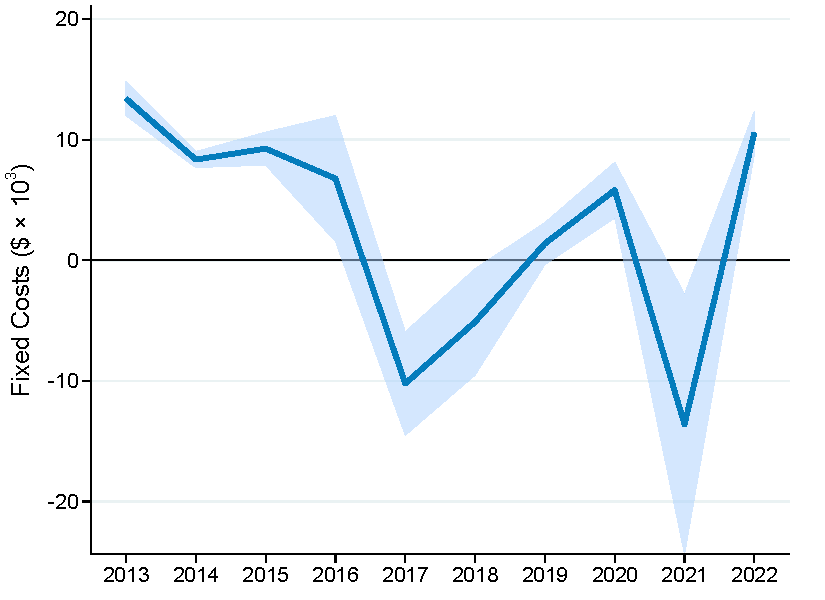
\includegraphics[width=\textwidth]{CA_SGIP/linear_fc.pdf}
\caption{Estimated value of $\alpha^{R}_{t}$ from Eq. \ref{eq:augustineblair2021} by year.}\label{fig:linear_fc}
\end{figure}

\begin{figure}[p]
\centering
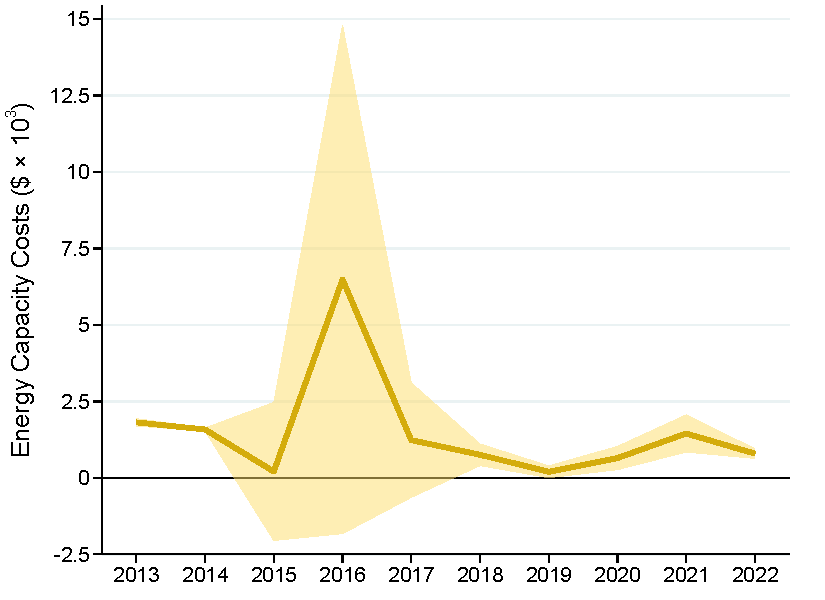
\includegraphics[width=0.9\textwidth]{CA_SGIP/linear_ecc.pdf}
\caption{Estimated value of $\beta_{1t}$ from Eq. \ref{eq:augustineblair2021} by year.}\label{fig:linear_ecc}

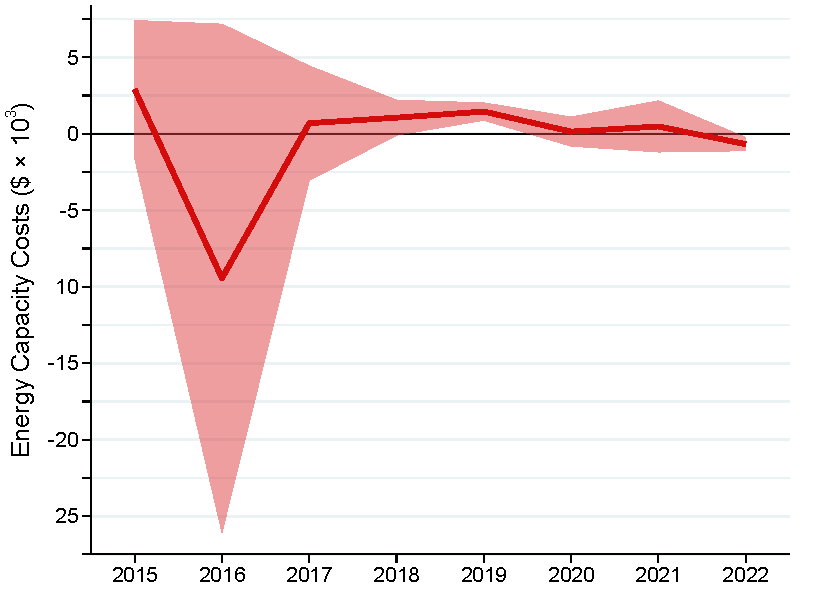
\includegraphics[width=0.9\textwidth]{CA_SGIP/linear_pcc.pdf}
\caption{Estimated value of $\beta_{2t}$ from Eq. \ref{eq:augustineblair2021} by year.}\label{fig:linear_pcc}
\end{figure}